\section{Experiments}
\begin{figure}
  \centering
  \begin{subfigure}[b]{0.48\linewidth}
    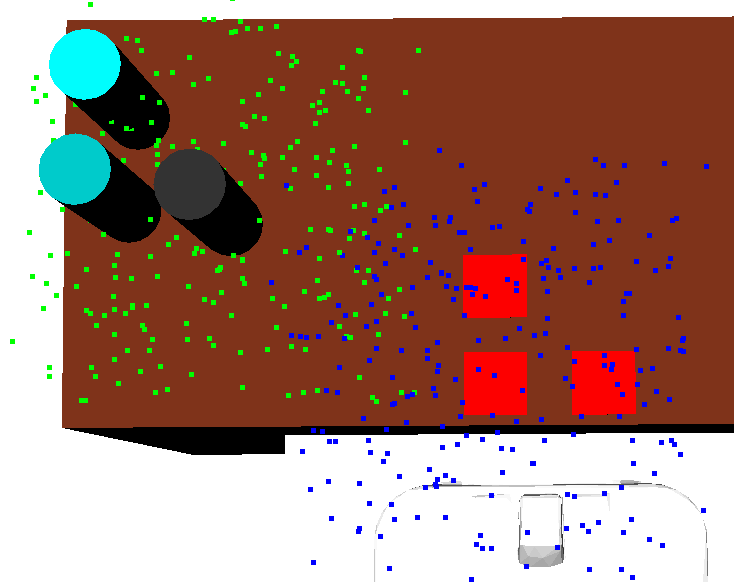
\includegraphics[width=\textwidth]{images/learns.png}
    \caption{Initial distribution}
  \end{subfigure}
  \begin{subfigure}[b]{0.48\linewidth}
    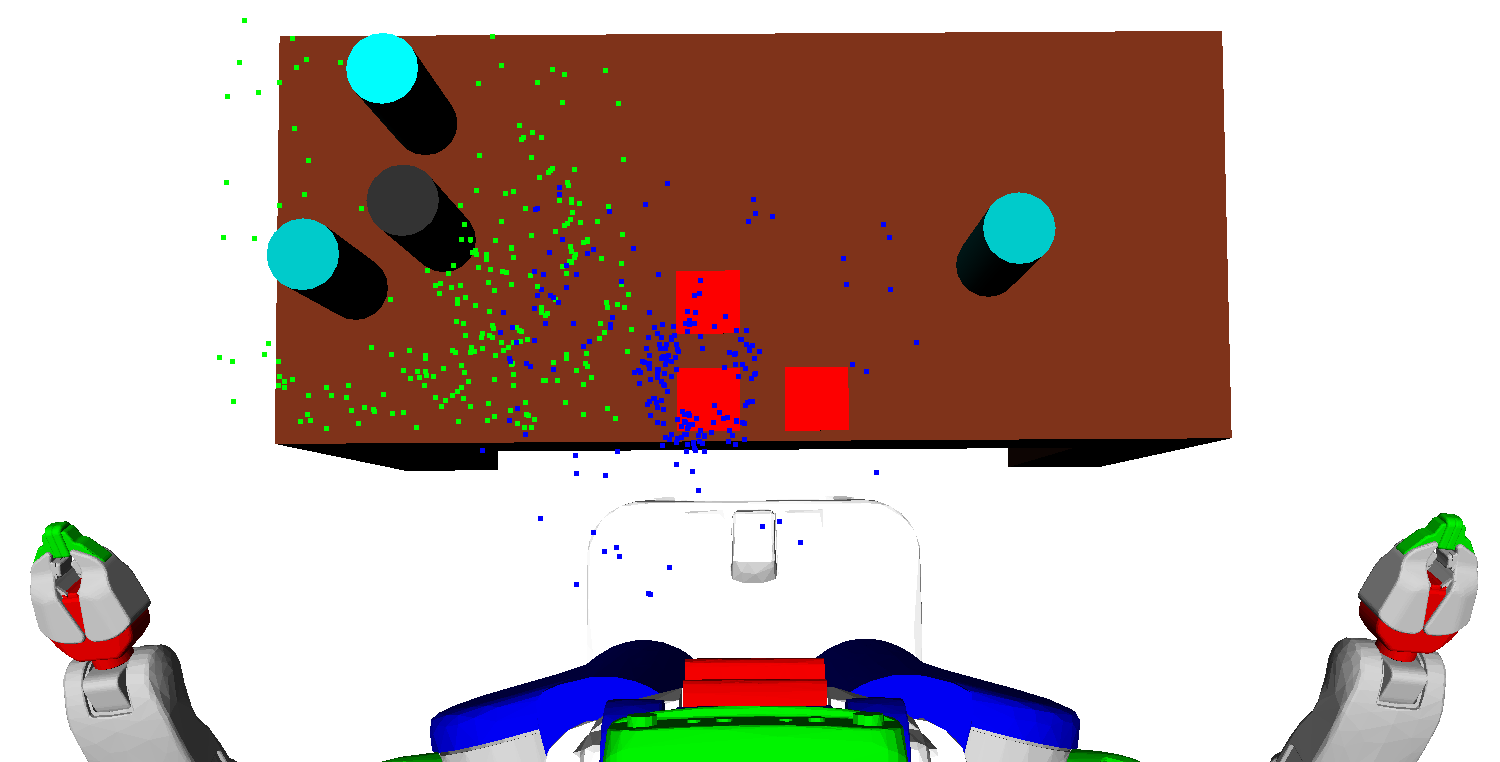
\includegraphics[width=\textwidth]{images/learn10.png}
    \caption{After 10 iterations.}
  \end{subfigure}
  \begin{subfigure}[b]{0.48\linewidth}
    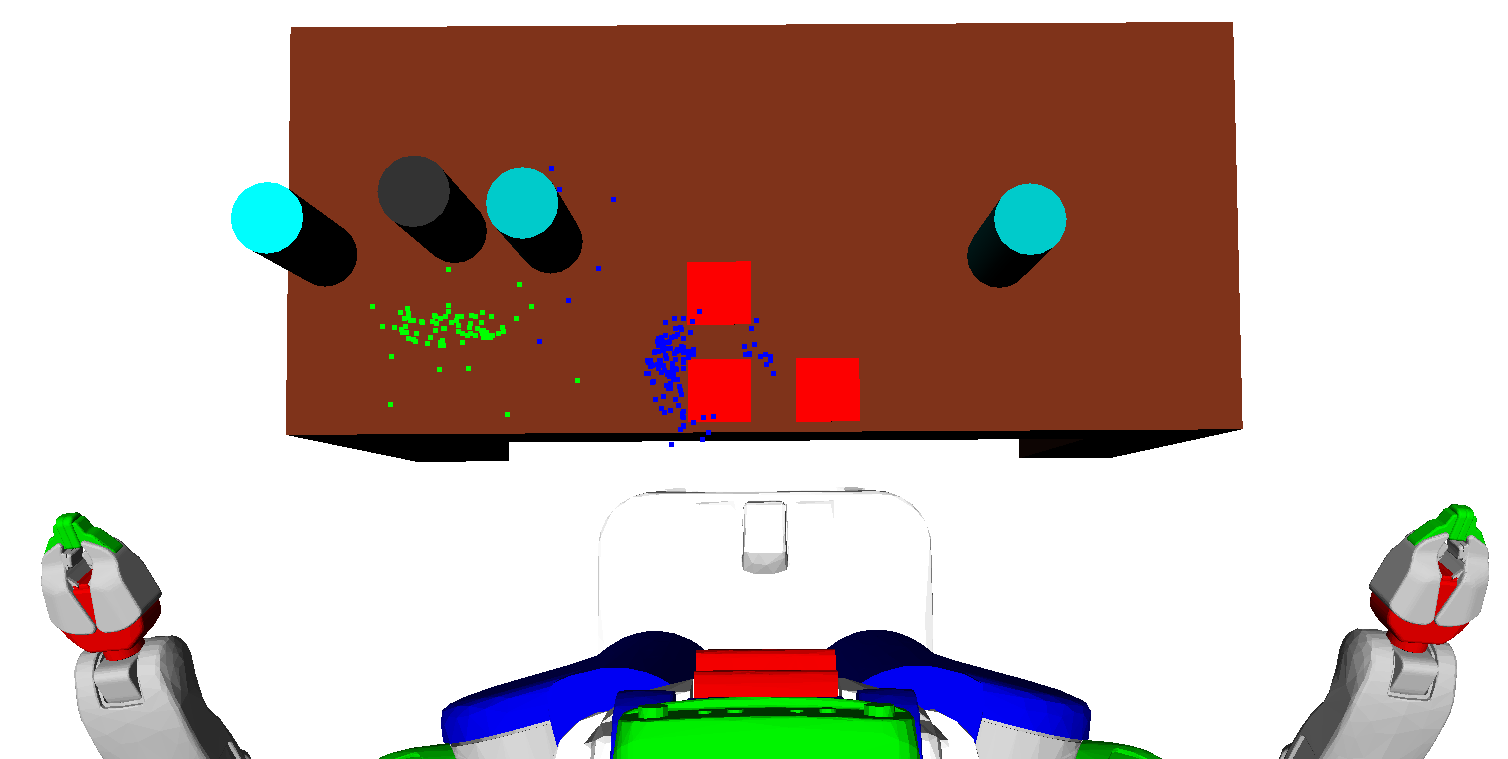
\includegraphics[width=\textwidth]{images/learn15.png}
    \caption{After 15 iterations.}
  \end{subfigure}
  \begin{subfigure}[b]{0.48\linewidth}
    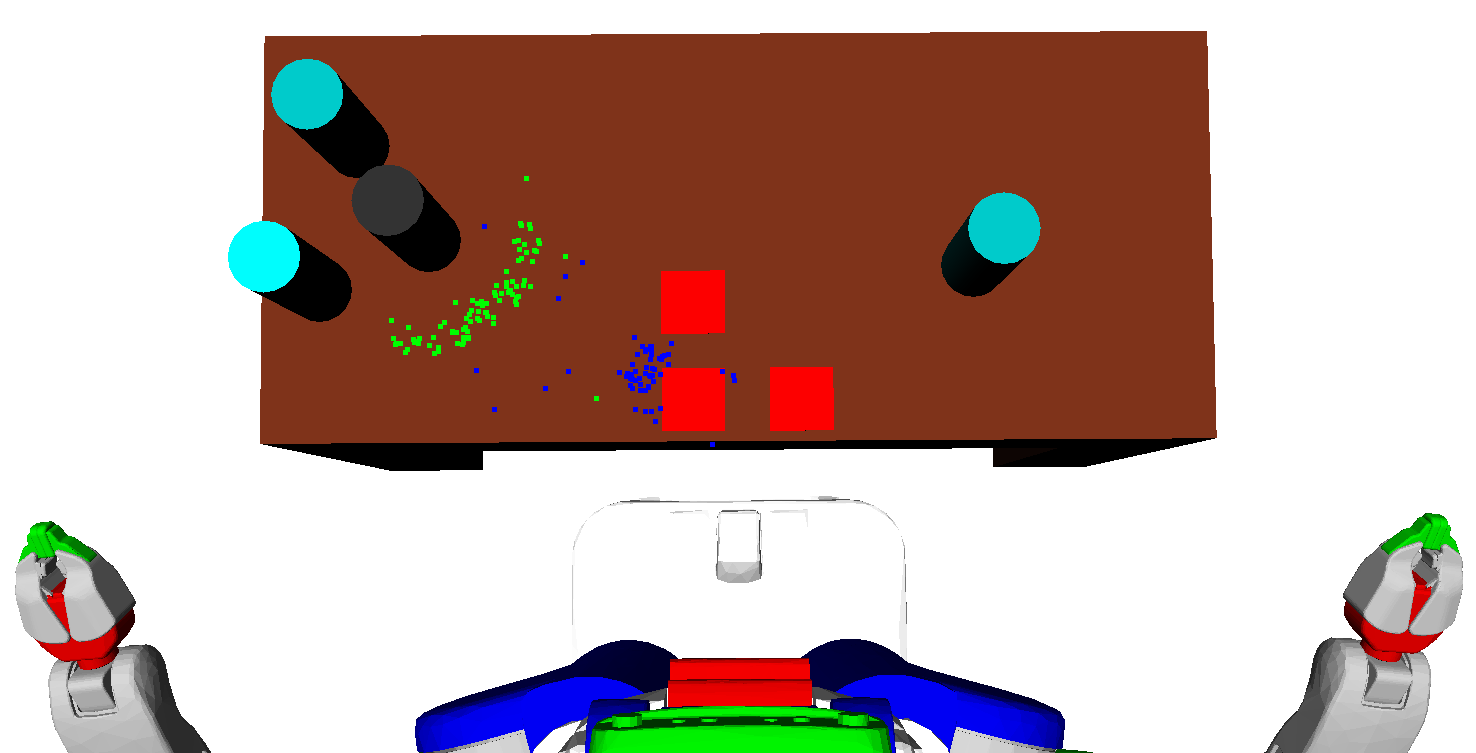
\includegraphics[width=\textwidth]{images/learn20.png}
    \caption{Final distribution.}
  \end{subfigure}
  \caption{Learned left arm grasp (green) and putdown (blue) distributions used to
pick up the black can and place it on the central red square, after different training iterations.
An iteration refers to a single run of randomized refinement,
which terminates after $L$ calls to the \texttt{resample} routine. The
initial distributions are uniform because we initialize weights to $\vec{\mathbf{0}}$.
The final distributions are after 20 iterations. The convergence and robustness of
the distributions demonstrate the soundness of our approach.}
  \label{fig:training}
\end{figure}

\begin{figure}
  \centering
  \begin{subfigure}[b]{0.3\linewidth}
    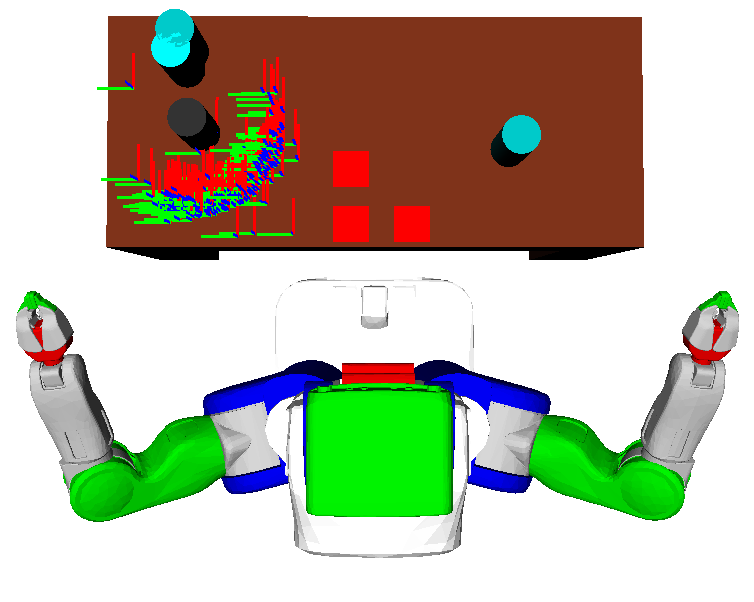
\includegraphics[width=\textwidth]{images/finalgraspnoobstr.png}
    \caption{}
  \end{subfigure}
  \begin{subfigure}[b]{0.3\linewidth}
    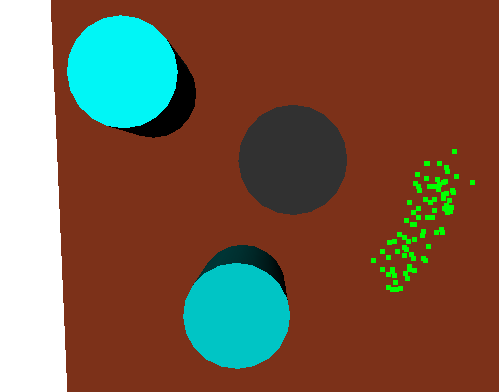
\includegraphics[width=\textwidth]{images/finalgraspobstr.png}
    \caption{}
  \end{subfigure}
  \begin{subfigure}[b]{0.3\linewidth}
    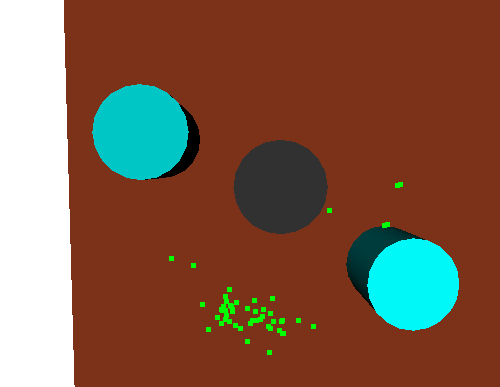
\includegraphics[width=\textwidth]{images/finalgraspobstr2.png}
    \caption{}
  \end{subfigure}
  \caption{The learned grasp pose distribution
is shown with different obstruction layouts. The system learns to
avoid obstructions while providing a good set of grasping poses.}
  \label{fig:obstr}
\end{figure}

\begin{table}
  \centering
  \vspace{8pt}
  \tabcolsep=0.11cm{
  \begin{tabular}{ccccc}
    \toprule[1.5pt]
      \textbf{System} & \textbf{Experiment} & \textbf{\% Solved} & \textbf{Avg MP Time (s)} & \textbf{Avg \# MP Calls}\\
    \midrule[2pt]
      B & 1, 1 obstr & 100 & 8.16 & 18.93\\
    \midrule
      L & 1, 1 obstr & 96 & 6.11 & 11.5\\
    \midrule[1.5pt]
      B & 1, 2 obstr & 96 & 8.74 & 19.7\\
    \midrule
      L & 1, 2 obstr & 94 & 12.26 & 20.77\\
    \midrule[1.5pt]
      B & 1, 3 obstr & 84.44 & 10.77 & 23.16\\
    \midrule
      L & 1, 3 obstr & 97.78 & 10.6 & 19.1\\
    \midrule[1.5pt]
      B & 2 & 33.33 & 12.1 & 21.1\\
    \midrule
      L & 2 & 96.67 & 9.19 & 17.78\\
    \midrule[1.5pt]
      B & 3 & 100 & 4.52 & 12.24\\
    \midrule
      L & 3 & 100 & 5.94 & 15.36\\
    \bottomrule[1.5pt]
  \end{tabular}}
  \caption{Percent solved, along with time spent motion planning and number of calls to the motion
planner for the final refinement. Results are averaged across 50 test environments per experiment, when both
the baseline and our system succeed. The test environments were grouped into 10 batches of 5, and
each batch received independent training with a distinct random seed. For each experiment,
we provide baseline system results using hand-tuned sampling distributions (B) and results from running
our system (L).}
  \label{table:results}
\end{table}

We evaluate our approach in several pick-and-place
tasks, varying the number of obstructions, obstruction locations, and whether
the base is allowed to move. We compare performance with that of the
hand-coded sampling distributions used in Srivastava et al.~\cite{srivastava2014combined}.
In this work, our training focuses on the problem of refining a single high level
plan. However, during actual planning, we may start with a high level plan that
has no valid refinement, and symbolic error information must be propagated to the
task planner, which produces a new plan. In future work, we will
incorporate this into the learning framework, but for now we measure performance
only on the refinement of the final high level plan.

We use the reward function described earlier. Our weight
vectors are initialized to $\vec{\mathbf{0}}$ for all parameter types.
This initialization represents a uniform distribution across the limits of the geometric search space.
Our domain has 3 types of continuous parameters: base poses, object grasp poses, and object putdown poses.
The range of allowable values for grasp and putdown poses is a cube of side length 30 centimeters
around the target object or putdown location. For base poses, the range is a
square of side length 1 meter around the object or location which the robot is approaching.
We use 24 features. 9 binary features encode the bucketed distance between the sample
and target. 9 binary features encode the bucketed sample height. 3 features
describe the number of other objects within discs of radius 7, 10, and 15 centimeters around the
sample. 3 binary features describe the angle made between the vector from the
robot to the target and the vector from the sample to the target: whether the angle is less than
$\pi/3$, $\pi/2$, and $3\pi/4$.

Our experiments are conducted in Python 2.7 using the OpenRave simulator~\cite{Diankov_2008_6117} with a PR2 robot.
The motion planner we use is trajopt~\cite{schulman2013finding}, and the task planner is Fast-Forward~\cite{FF}.
The experiments were carried out in series on an Intel Core i7-4770K machine
with 16GB RAM.

We train and test 3 different experiments, all of which share a common goal of
grasping a target object from a table and putting it down at a specific location on the table.
The locations of the obstructions surrounding the target object were
sampled uniformly from a thick ring around the object with inner radius 0.13 meters
and outer radius 0.25 meters. Table \ref{table:results} summarizes our quantitative results.
\figref{fig:cover} plots learned distributions for a move-grasp-move-putdown sequence of actions.
\figref{fig:training} illustrates the training of grasp and putdown distributions, and \figref{fig:obstr}
shows how the learned grasp distribution interacts with obstructions.

\textbf{Experiment 1}: Grasp is obstructed by 1 through 3 objects; no base motion.
$N = 20$, $L = 16$, $\epsilon = 4$. Our system outperforms the baseline for both 1 and 3
obstructions, but performs worse for 2. We attribute this to the fact that random seeding can
have a huge effect on which local optimum our policy gradient algorithm finds. An additional
observation is that motion planner time and number of calls are not always linearly related; some target
poses may be IK feasible but difficult to reach, causing the motion planner to take longer
to find a trajectory.

\textbf{Experiment 2}: Putdown is obstructed in cardinal directions; no base motion.
$N = 20$, $L = 16$, $\epsilon = 4$. This is a contrived example to illustrate the
issues with coarse discretization of the sample space.
The baseline system only attempts putdown pose instantiation in the
4 cardinal directions, explaining the large performance disparity.

\textbf{Experiment 3}: Grasp is obstructed by 1 object; base motion allowed.
$N = 60$, $L = 100$, $\epsilon = 20$. Our system performs slightly worse than the baseline
here, but not significantly. We believe this is because more time is spent motion planning
base poses from which grasps and putdowns are infeasible (since candidate base poses are no
longer hand-engineered), triggering resampling of the value assigned to the base pose parameter.
